\documentclass{beamer}

\setbeamertemplate{title page}[default][left] % left-align title page (commend out for centered title page)
\beamertemplatenavigationsymbolsempty % remove navigation symbols

\input{preamble}

\title{De-novo canonical miRNAs}
\subtitle{A pilot study including iterative models}
\author{Cristian A. Velandia H}
\institute{TBI \\ University of Vienna}
\email{cavelandiah@tbi.univie.ac.at}
\date{}


\begin{document}

\begin{frame}
    \maketitle
\end{frame}

% Include individual or combined slides.
%\include{slides/example}
%\include{slides/example-julia-console}
%\include{slides/example-plotting}
%\include{slides/example-tikz}
%\include{slides/example-algorithm}
%\include{slides/example-definition}
%\include{slides/example-table}
%\include{slides/example-bullets}

\begin{frame}[t]
    % Take the most expressed candidates from the 24 ones and show one comparison.
    \frametitle{microRNAs on \textit{Ciona robusta}}
    Chromosome $7$ cluster ($28$ miRNA loci over $3713$ nt)
    \begin{figure}[h!]
        \centering
        \includegraphics<1>[width=\linewidth]{Figures/chr7_cluster} %
        \includegraphics<2>[width=\linewidth]{Figures/mor_example} %
    \end{figure}
    \begin{itemize}[<+->]
        \item Annotations without `miR-family' classification.
        \item Prevalence of miRNA-offset (moR) (adjacent to miR/miR*).
    \end{itemize}
\end{frame}

\begin{frame}[t]
    % Take the most expressed candidates from the 24 ones and show one comparison.
    \frametitle{microRNAs on \textit{Ciona robusta}}
    Homology annotation using \texttt{miRNAture} + \texttt{miRBase}: low coverage.
    \begin{figure}[h!]
        \centering
        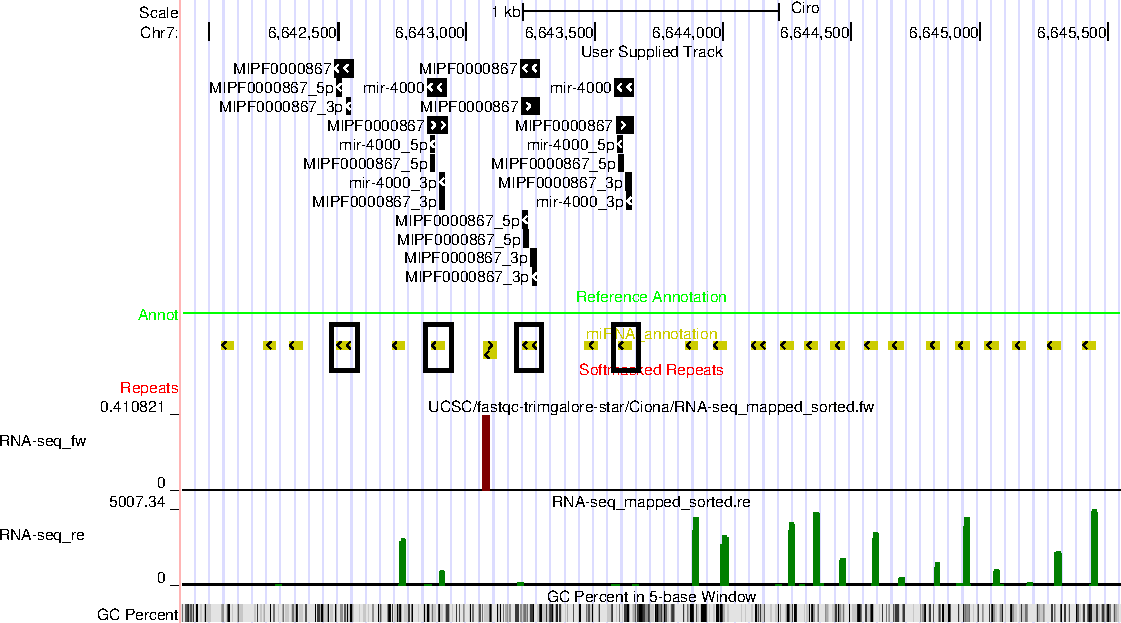
\includegraphics[width=\linewidth]{Figures/homology_coverage} %
    \end{figure}
\end{frame}

\begin{frame}[t,label=problem5]
%\begin{frame}{Algorithms}
    \frametitle{\textit{De novo} miRNA annotation on \textit{Ciona robusta}}
    \framesubtitle{Re-analysis small RNA-seq data}
    \begin{table}[h!]
        \centering
        \caption{Available SRA small-RNA/miRNA-seq for \textit{C.\ robusta}: $3$ experiments ($X$ libraries)}
        \label{tab:experiments}
        \begin{tabular}{llp{1cm}}
            \toprule
            \textbf{Run} & \textbf{Experiment} & \textbf{Lib.} \\ \midrule
            SRP002173 & small-RNA for two developmental stages & $X$ \\ %& Shi W, Hendrix D, Levine M. \\
            SRP079886 & Expression Oral Siphon Regeneration & $Y$ \\ %& Spina EJ, Guzman EB, et al. \\
            SRP116990 & small-RNA transgenic ascidians & $Z$ \\ %& Suntory Foundation \\
            \bottomrule
        \end{tabular}
    \end{table}
    \begin{figure}[h!]
        \centering
        \includegraphics<1>[width=0.7\linewidth]{Figures/solitarytunicate.png} %
        \caption{\textit{C.\ robusta}. Source: $X$}
    \end{figure}
\end{frame}

\begin{frame}[t]
    \frametitle{From motifs to blocks}
    \framesubtitle{Discovering \textit{de-novo} miRNAs}
    \begin{figure}[h!]
        \centering
        \includegraphics<1>[width=0.55\linewidth]{Figures/workflow} %
        %\includegraphics<2>[width=\linewidth]{Figures/deNovoMethod2}\label{fig:synteny1497} %
        %\includegraphics<3>[width=.7\linewidth]{Figures/denovopositive} %
        %\includegraphics<4>[width=.7\linewidth]{Figures/denovopositive2}    
    \end{figure}
\end{frame}

\begin{frame}[t]
    \frametitle{Results: Canonical refining}
    \framesubtitle{Discovering \textit{de-novo} miRNAs}
    \begin{figure}[h!]
        \centering
        \includegraphics<1>[width=\linewidth]{Figures/results_workflowALL}\label{fig:workflow} %
        \includegraphics<2>[width=0.55\linewidth]{Figures/isomir_example2}\label{fig:workflow} %
    \end{figure}
    \begin{itemize}
        \item<1>[-] Only $3.6$\% candidates detected as \textit{canonical} miRNAs.
        \item<2>[-] Mostly short candidates: maturation by-products?/isomirs? ($\sim 77.4$\%)
    \end{itemize}
\end{frame}

\begin{frame}[t]
    % Take the most expressed candidates from the 24 ones and show one comparison.
    \frametitle{Results: Going back to Chr7 cluster}
    Canonical de-novo families: One additional candidate on Chr7 $:($
    \begin{figure}[h!]
        \centering
        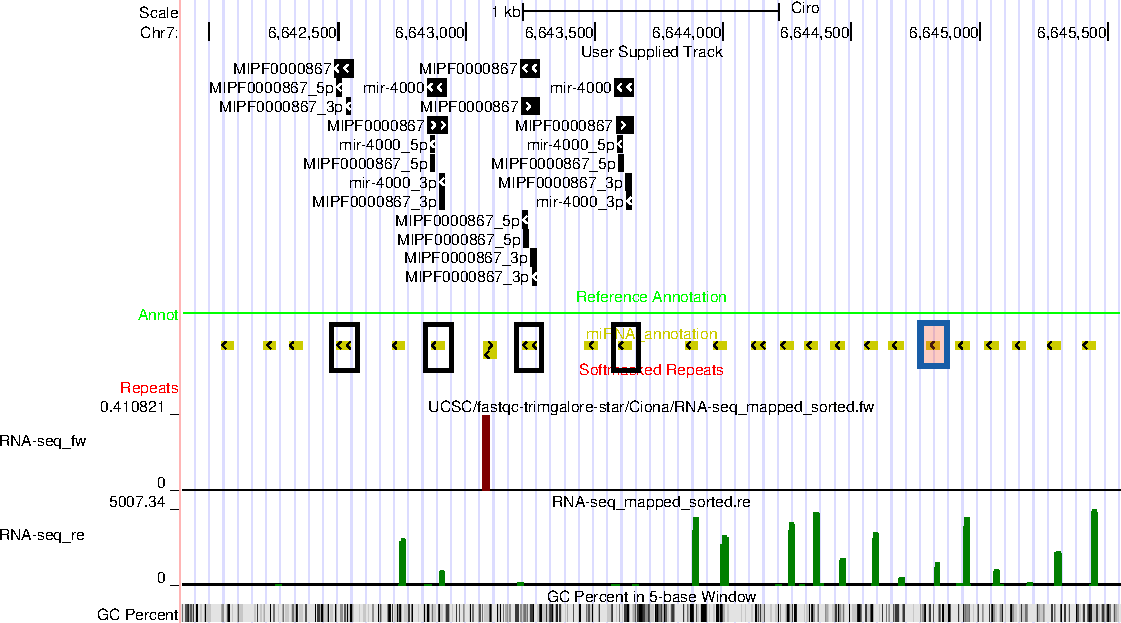
\includegraphics[width=0.9\linewidth]{Figures/homology_coverage_denonvo} %
    \end{figure}
    \textbf{Why $\sim82$\% loci were not detected?} 
\end{frame}

\begin{frame}[t]
    % Take the most expressed candidates from the 24 ones and show one comparison.
    \frametitle{Results: miRNA annotation on chordates}
    \begin{figure}[h!]
        \centering
        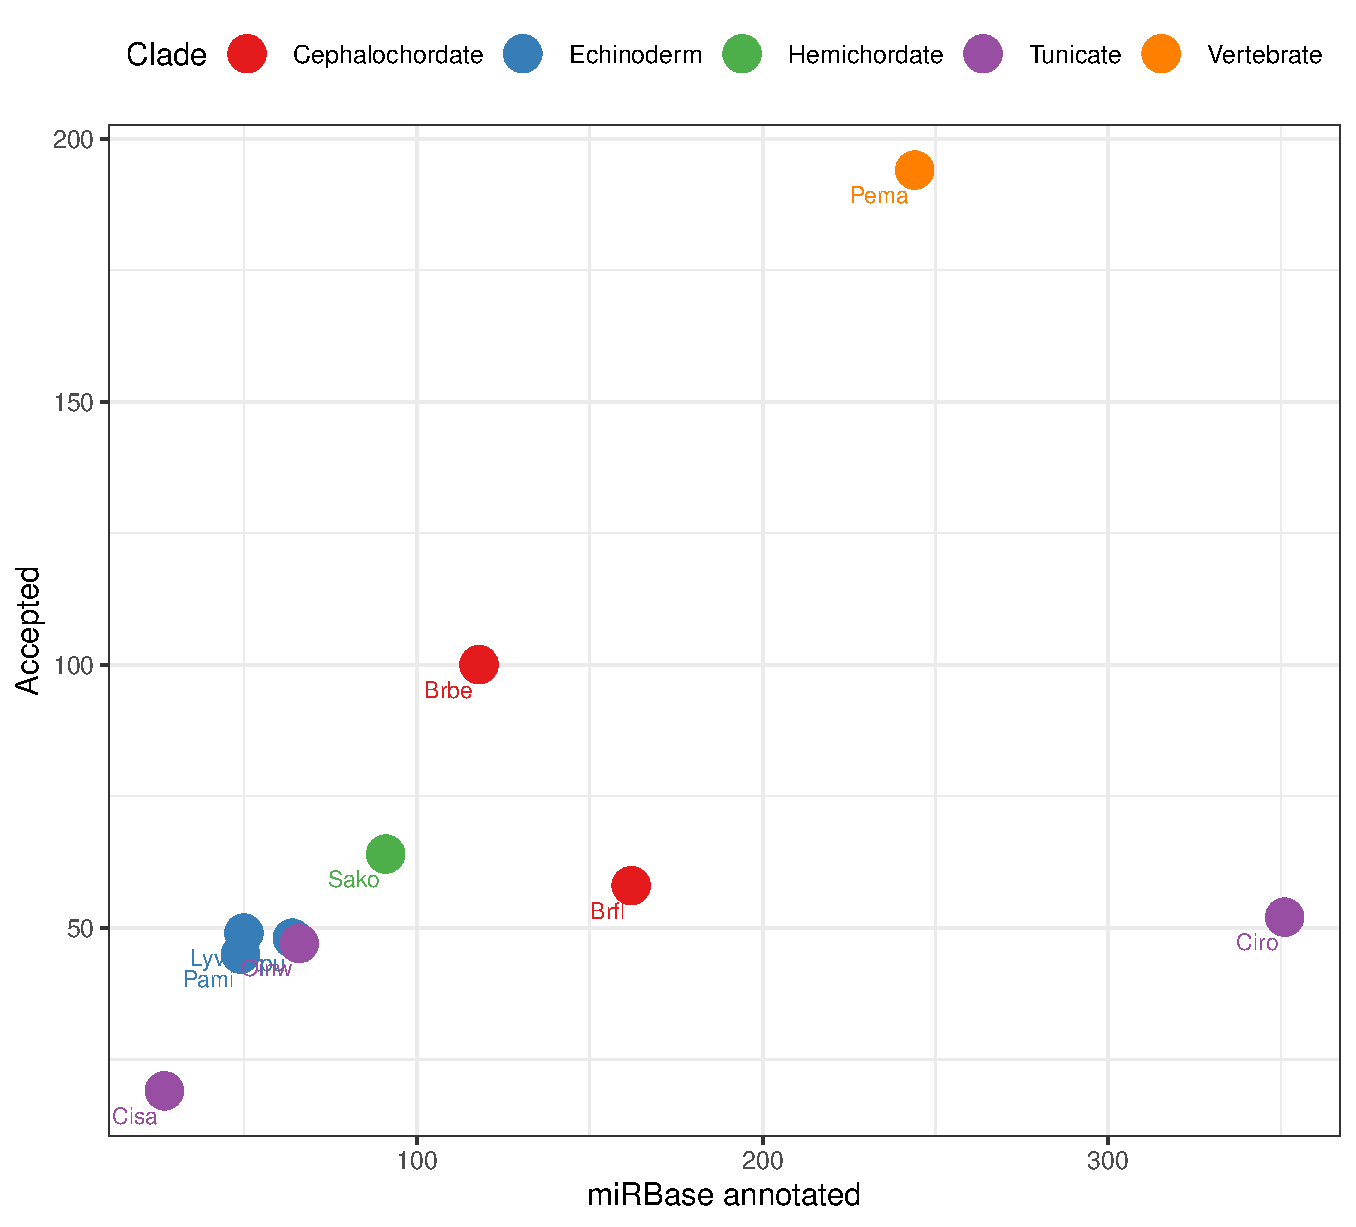
\includegraphics[width=.45\linewidth]{Figures/annotated_vs_accepted} %
    \end{figure}
    \begin{itemize}[<+->]
        \item \textit{C.\ robusta} annotations: $351$ loci
        \item With Fam.: $18.5$\% / No Fam: $81.5$\%.
        \item $13\times$ than sister specie: \textit{Ciona savignyi}
        \item Higher loci number than coelacanth and lancelet (!).
    \end{itemize}
\end{frame}

\begin{frame}[t]
    % Take the most expressed candidates from the 24 ones and show one comparison.
    \frametitle{Results: Discovering canonical miRNAs}
    Finding canonical de-novo families: Structural assessment
    \begin{figure}[h!]
        \centering
        \includegraphics<1>[width=\linewidth]{Figures/evaluation_annotation_mirbase1} %
        \includegraphics<2>[width=\linewidth]{Figures/evaluation_annotation_mirbase2} %
        \includegraphics<3>[width=\linewidth]{Figures/mor_example} %
    \end{figure}
     \begin{itemize}[<+->]
         \item Canonical miRNAs represent $\sim21$\% of cluster.
         \item Reasons: Position of mature sequences on loop regions, structural constrains, miRNA-offset.
     \end{itemize}
\end{frame}

%\begin{frame}[t]
%    \frametitle{Results: Iteration $1$}
%    \framesubtitle{Discovering \textit{de-novo} miRNAs}
%    \begin{itemize}
%        \item Starting point: $24$ CMs from \textit{C.\ robusta}.
%        \item First target specie: \textit{Ciona savignyi}.
%    \end{itemize}
%\end{frame}

\begin{frame}[t]
    \frametitle{Conclusions}
    \begin{itemize}
        \item Non-trivial miRNA annotation (i.e simplified chordate $\sim120$ Mb genome).
        \item Need to extend \texttt{miRNAture} \& \texttt{MIRfix} to non-canonical miRNAs/expression products associated to microRNA maturation.
        \item Iterative models for miRNAs: expression patterns (blocks, clusters), mature definition, mature position, structural assessment, evolutionary information (+ synteny?).
    \end{itemize}
\end{frame}

\begin{frame}[t]
    % Take the most expressed candidates from the 24 ones and show one comparison.
    \frametitle{Appendix: miRNA annotation on chordates}
    \begin{figure}[htpb]
        \centering
        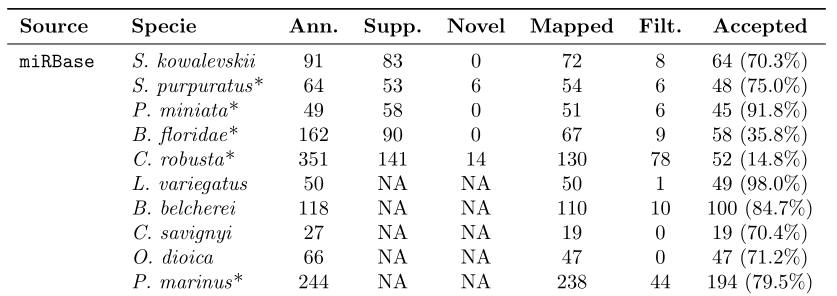
\includegraphics[width=\textwidth]{Figures/support_mirbase_table.png}
        %\caption{miRNA annotation on selected chordates}
        \label{fig:chordatesann}
    \end{figure}
\end{frame}



%\begin{frame}{References}
%    \printbibliography
%\end{frame}

\end{document}
